\section{Background into Classic Methods}



Features in data are often colloquially spoken of but rarely have rigorous descriptions. We will look at a common dataset to illustrate how features express them selves: The "Iris Dataset"\cite{Iris:Fisher} . This dataset is an excellent playground to bridge the gap between statistical intuition and formal analysis on higher dimensional data. The Iris flower has been formally studied by botanists since 1913.The successful husbandry of these flowers are highly dependent on which species are in the genetic pool a botanist is drawing from. In Fishers 1934 paper "The use of multiple measurements in taxonomic problems" \cite{Iris:Fisher} it was surprising to observe a third species in what was previously thought to be a two species data set. This dataset was created by selecting 50 samples of flowers from each of the three species sets Setosa, Versicolor, and Virginica. With each sample, four properties were measured. The final makeup of the data set is 150 samples with 5 properties: petal length, petal width, sepal length, sepal width, and species. In the following description we will see that the species can be made dependent on the other 4 properties. 

\begin{wrapfigure}{r}{0.4\textwidth}
\centering
    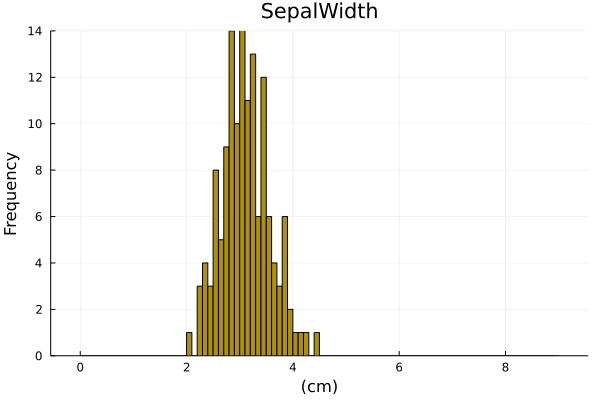
\includegraphics[width=0.35\textwidth]{Code/SepalWidthTotHist.png}
    \caption{Histogram of sepal width from the Iris dataset}
    \label{fig:SepalWidthTotHist}
\end{wrapfigure}
Distributions and histograms are ubiquitous in any scientific analysis, but for emphasis it bears repeating here. A \emph{histogram} is constructed by counting the frequency a property in a dataset obtains a certain value (or range of values). For example in Fig. \ref{fig:SepalWidthTotHist}. the property sepal width is binned into bins of 1 mm width between 0 and 9 cm. The histogram tells us that sepal width is roughly between 2cm and 5cm with a large concentration at about 3 cm. Finally, one may also observe that the histogram is roughly the shape of a bell curve. These are interesting qualitative features to observe, but more importantly, this histogram, after normalizing, is an approximation to a \emph{probability distribution}. In a subject matter specific setting, exactly the distribution that this data is drawn from would be hotly contested based on expert testimony of what could be driving the variation.
\begin{wrapfigure}{l}{0.4\textwidth}
\centering
    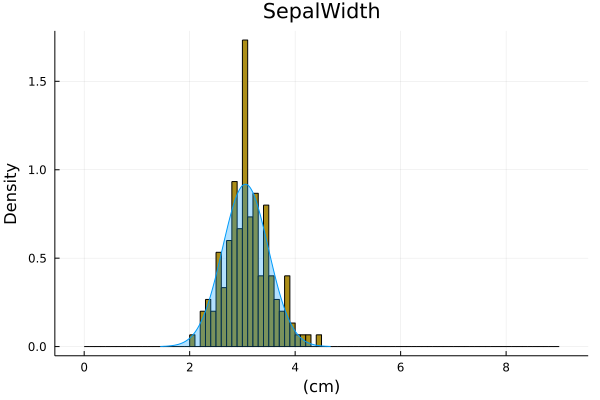
\includegraphics[width=0.35\textwidth]{Code/SepalWidthTotHistFit.png}
    \caption{Normalized histogram with fitted probability density overlay }
    \label{fig:SepalWidthTotHistFit}
\end{wrapfigure}

For demonstration purposes, assume that the physics, chemistry, and biology cause sepal width to be drawn from a normal distribution. The probability density function for a normal distribution is the Gaussian function. After normalization, the gaussian can be parameterized by two values: The \emph{mean}, which is also called the \emph{expected value}, and the \emph{variance} which is related to the \emph{standard deviation}. In Fig. \ref{fig:SepalWidthTotHistFit} a normal distribution has been fit to the sepal width and overlayed on top of the normalized histogram. While this example may be overly pedantic, \textbf{it is important to note that the algorithm to fit a single gaussian is brute force arithmetic of computing the mean and variance}. The fitted normal distribution gives a model by which to compare and measure new data against. So far the sepal width data has not given any profound insights. At most, if a graduate student was sent to the green houses to measure flowers and they came back with many samples of lengths around 6cm, you could compute the \emph{log likelihood} and quantitatively see that the graduate student did not know the difference between an Iris and, say, a Lili. The usefulness of this model is marginal. However, all is not lost, there are still 3 more properties to analyze and extract meaningful insight.
\begin{figure}[h]
\centering
    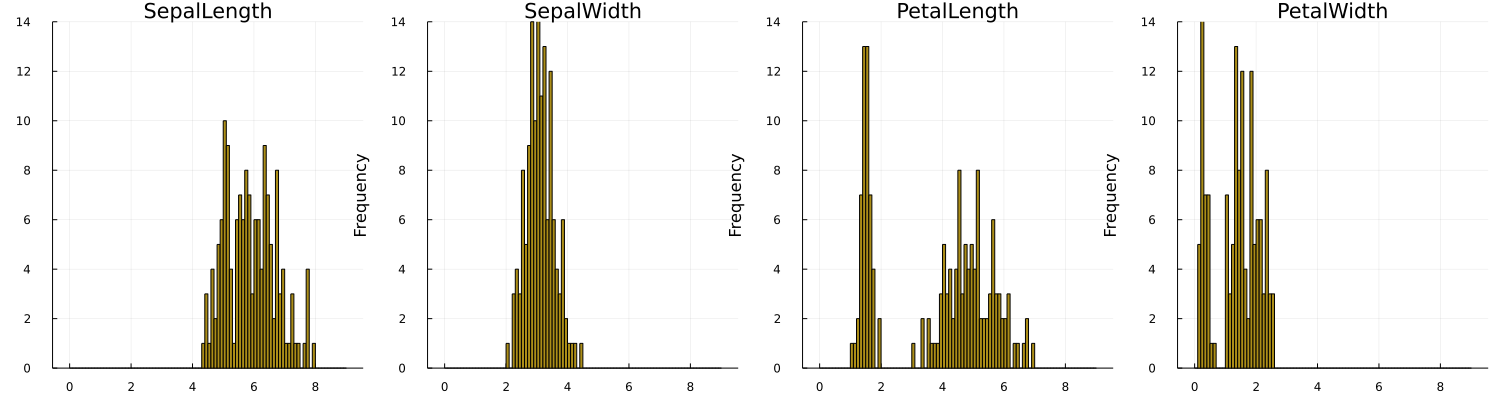
\includegraphics[width=1.0\textwidth]{Code/propHist4x1_tot.png}
    \caption{Histograms of each of the 4 properties measured in the Iris dataset }
    \label{fig:propHist4x1_tot}
\end{figure}
Let us examine the histograms of all properties in Fig. \ref{fig:propHist4x1_tot}. If one tries to fit a Gaussian function to the remaining properties, the error from sepal length will be modest, however the error from fitting gaussian to petal length or petal width will be significantly more. Or in other words, a normal distribution is a bad model for petal length and petal width. A blind approach to find a good model would be to try popular classic distribution like a beta, gamma, or exponential  distribution. Unfortunately, these will suffer from the same bad error that a normal distribution did. More exotic models are required. There is no full-proof standard way of choosing an optimal model \footnote{If we made assumptions about the underlying causality of what is driving this data we could indeed choose a class of models or even a specific parameterized model}. As uncomfortable as it may be, this is where science becomes an art, and also the root of why it is so hard to define an abstract and formal definition of a \emph{feature in data}. Many human brains may look at the petal length and width histograms and see two vague curves in each. This is inspiration enough to choose a Gaussian Mixture Model (GMM). 


\begin{wrapfigure}{l}{0.5\textwidth}
\centering
    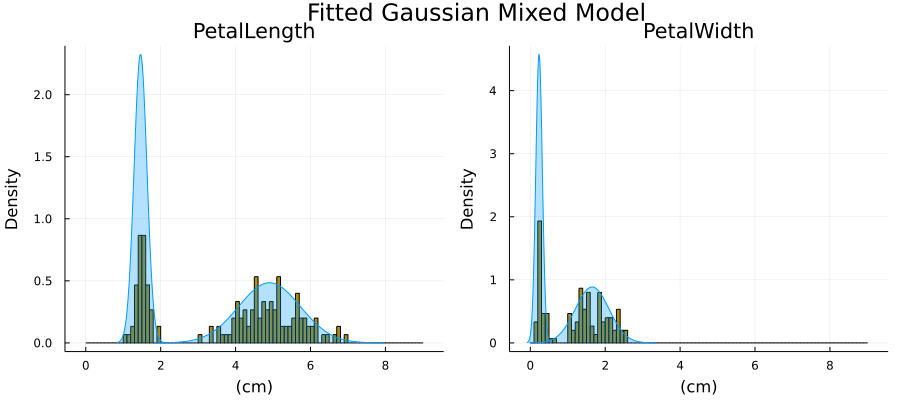
\includegraphics[width=0.5\textwidth]{Code/propHist2x1_OverTot.png}
    \caption{EM optimization initialized with means of 0, 5 and variance of 0.01, 0.1}
    \label{fig:propHist2x1_OverTot}
\end{wrapfigure}
There are many details to choosing and fitting the right GMM. In this case, there are three important details to explore. First, the mixture will contain two normal distributions. That means it is parameterized by a total of four parameters, two means and two variances. But, unlike a single normal distribution, computing the mean and variances to fit the model requires a more delicate approach. Second, It might feel like cheating for a human to choose a parameterized class of models (in this case, a two mode GMM), it is certainly cheating for a human to choose which subset of data they wish to compute the means and variances. Instead, the algorithm to fit the distribution using the entire dataset will be \emph{expectation maximization} (EM)\footnote{EM is considered a classic statistical leaning method. Because of its iterative nature, its spirit is very similar to more recent machine learning models and stochastic gradient decent.}.
\begin{wrapfigure}{r}{0.35\textwidth}
\centering
    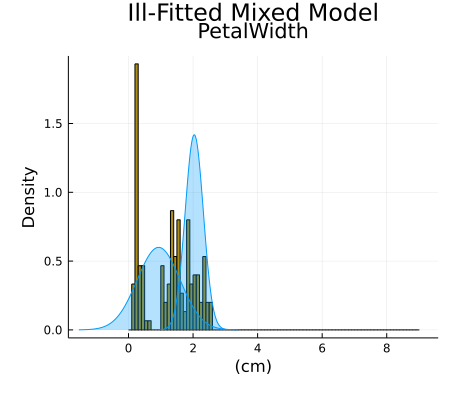
\includegraphics[width=0.35\textwidth]{Code/propHist2x1_OverTot_bad.png}
    \caption{EM optimization initialized with means of 0, 5 and variance of 0.1, 0.1. Resulted in poor fitting }
    \label{fig:propHist2x1_OverTot_bad}
\end{wrapfigure}
This algorithm can be roughly thought of as an iterative gradient method for optimizing the distributions parameters to achieve a best fit. Third, the EM algorithm can be very sensitive to the models initial parameters. Especially in one property dimension. Compare the difference between Fig. \ref{fig:propHist2x1_OverTot} and Fig. \ref{fig:propHist2x1_OverTot_bad}. With only a modest change in variance results in a reasonable fit in Fig. \ref{fig:propHist2x1_OverTot} and an absurd fit in Fig. \ref{fig:propHist2x1_OverTot_bad}.

In Fig. \ref{fig:propHist2x1_OverTot} there are acceptable fitted models to describe petal length and width. Petal length, qualitatively, has the more separated gaussian means between each lobe, let's focus on this property to identify the major object of interest, \emph{features in data}. Features in data are properties that can be measured. The goal of fitting an explicit model to the data is to create unambiguous values to make a measure against. To this end the fitted mixed models gives us explicit values for the means and variances of two Gaussians. We define features of this data with its model by measuring which gaussian each sample of data belongs to. Given a single example and using the formula for a gaussian, this can be done by computing the probability with respect to each gaussian. A feature will be assigned based on whichever probability is higher. Qualitatively, \emph{features in data} are subsets of data that can be "bunched together". Formally and abstractly, a feature in data is a subset that can be measured against some stochastic process like the example described above.

\begin{figure}[h]
\centering
    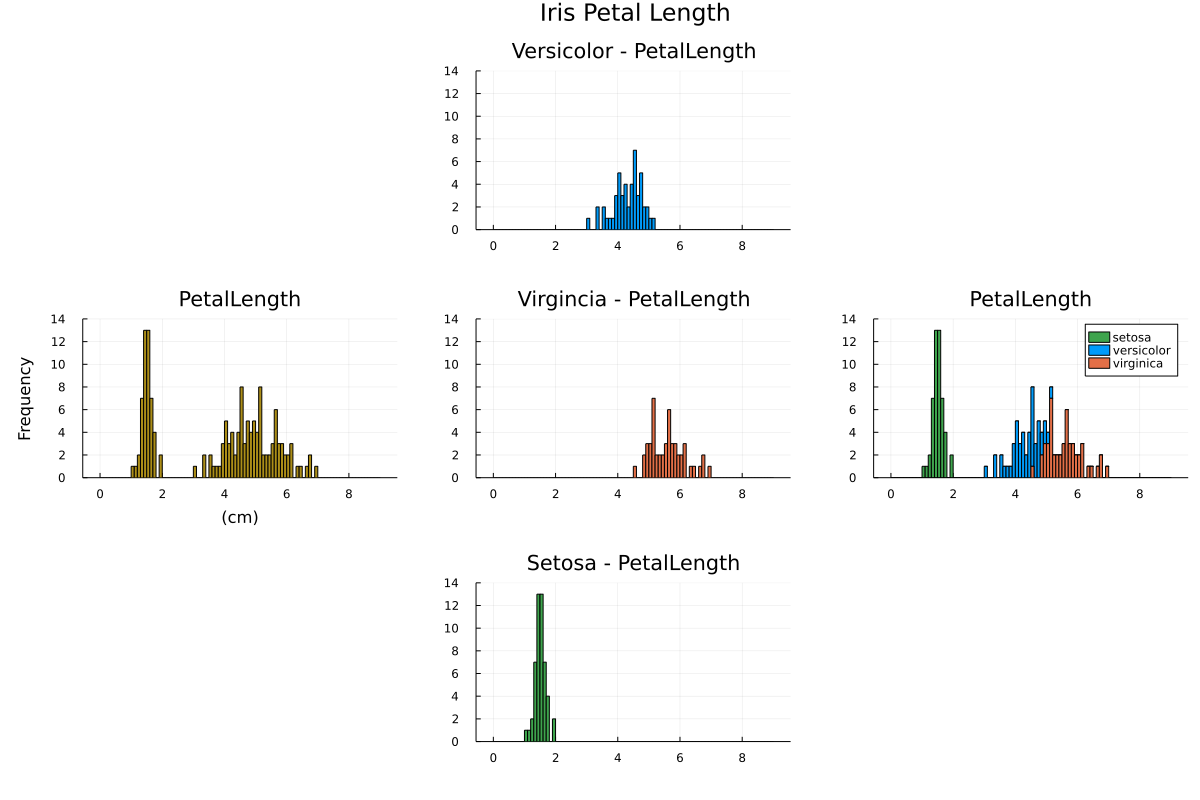
\includegraphics[width=1.0\textwidth]{Code/histBreakoutPetalLength.png}
    \caption{Breakout histograms of species }
    \label{fig:specBreakout}
\end{figure}

So far in this discusion, the features have no connection to reality. It is merely a curiosity that the data set has two statistically interesting features. This may lead one to perform further analysis of these samples. Indeed, in Fisher's paper \cite{Iris:Fisher} he describes that a mixture of husbandry practices and what are now known as early forms of genetic testing identify each sample with their genetic species. In figure Fig. \ref{fig:specBreakout} we reveal that the features in data that was discovered with the gaussian mixed model correspond to the Iris species Setosa in one feature, then versicolor and virginica in the second feature. It is important to note that in reality the genetics of the species causes, or implies, the length of petal. This discussion, however, focused on and found features in the data first, without having knowledge of the species, that can be used to guide further investigation by subject matter experts. This is the power of identifying features in data. The process of labeling data and finding features in data goes both ways.

The gaussian mixed model was able to isolate Setosa Iris as a feature. Even though the model was limited to 2 gaussians Fig. ref{fig:specBreakout} makes it clear that if a third was added the second and third gaussian would have struggle to fit the remaining species. This is a good opportunity to introduce join probability distributions and observe the importance of dimensionality. Features in data is also a story about dimensionality. A famous result in knot theory is "You can't tie your shoes in 4 dimensions". This is tragic for any aspiring high dimensional athletes, but good news for data scientists. 
\begin{wrapfigure}{l}{0.60\textwidth}
\centering
    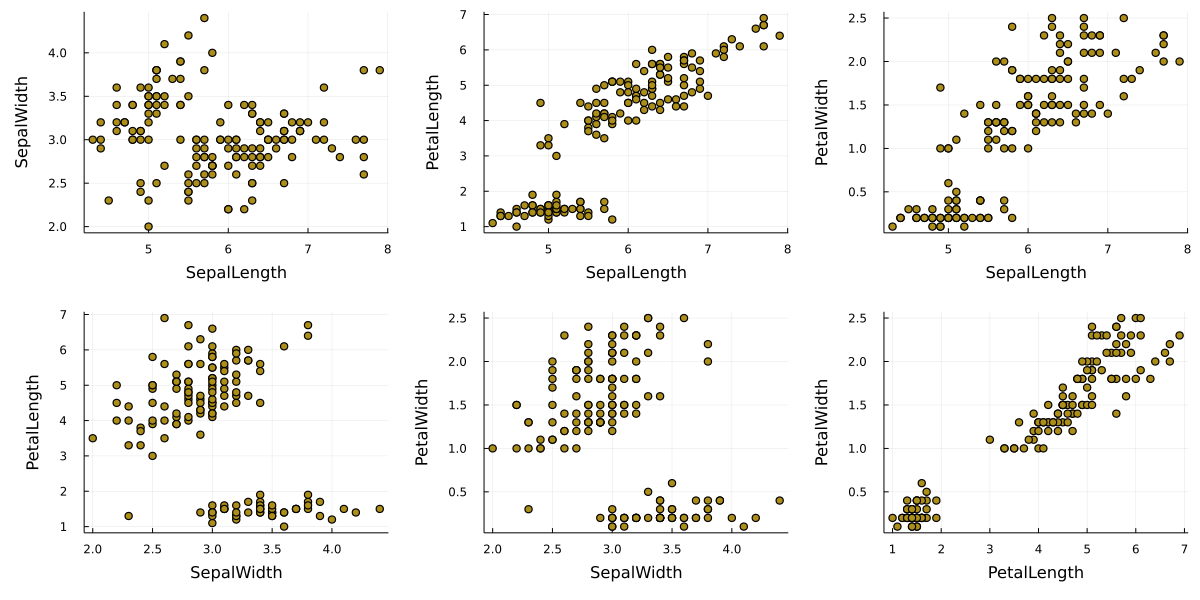
\includegraphics[width=0.60\textwidth]{Code/3by2PropVsPropUnLabeled.png}
    \caption{Estimations of join probability distribution of each pair of Iris properties}
    \label{fig:3by2PropVsPropUnLabeled}
\end{wrapfigure}
\begin{wrapfigure}{r}{0.60\textwidth}
\centering
    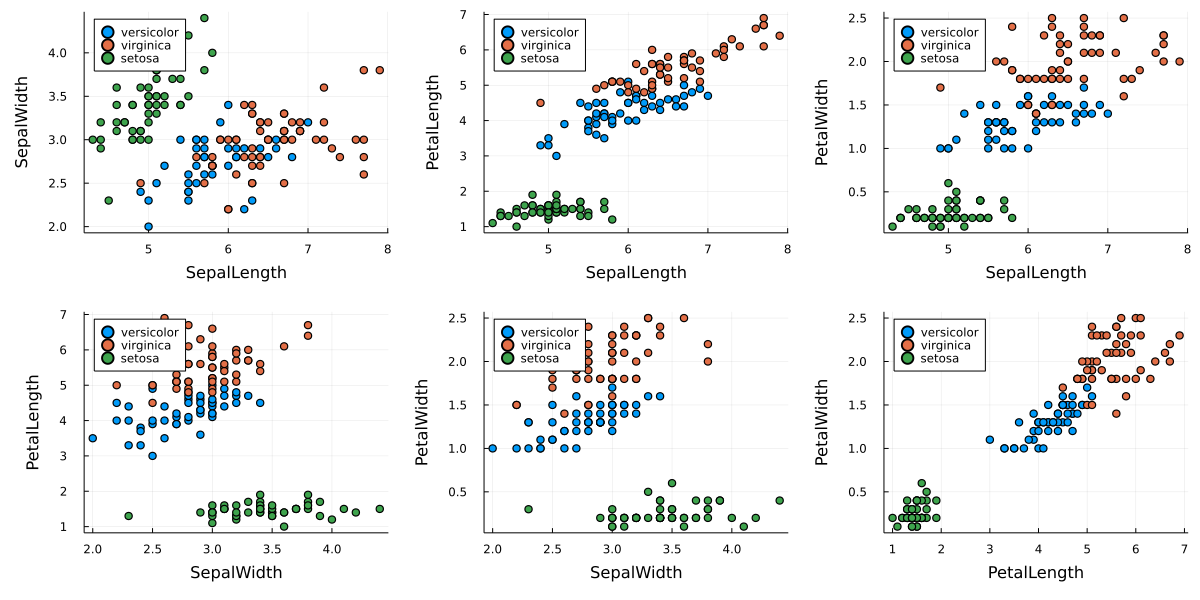
\includegraphics[width=0.60\textwidth]{Code/3by2PropVsPropLabeled.png}
    \caption{Estimations of join probability distribution of each pair of Iris properties}
    \label{fig:3by2PropVsPropLabeled}
\end{wrapfigure}
\emph{Joint probability distributions} in two properties is a function with two independent input variables and an output of a probability density for each pair of inputs. The scatterplots in Fig. \ref{fig:3by2PropVsPropUnLabeled} is not exactly a histogram or distribution. However, by partitioning the two dimensional domain into bins and counting the samples that are in each bin, one could imagine how these scatter plots represent an approximation to a distribution. It is important to note that the two dimensional domain is not as "full" as the one dimension domain. That is, if the domains were binned with, say, 1mm bins, the number of occupied bins is proportionally less in two dimensions than in one. \textbf{To properly sample higher dimensional spaces requires $O(p^n)$ more samples}. One can also observe samples bunching together creating areas of higher density.  The lessons learned from the one dimensional gaussian mixed model can be applied here, albeit with more parameters. Indeed, a multivariate normal distribution is parameterized by a \emph{mean} and \emph{variance} but the mean will be a $1 \times n$ vector and the variance will be a $n \times n$ matrix. Each item in the mean vector will be the simple mean that corresponds with its positions variable, but the variance matrix is made up of the variance and covariance of every variable measured agains every other variable. It is beyond the scope of this manuscript to go into depth about the specific meaning of these parameters, but the message that should be leaned here is \textbf{as dimensionality increases, so does the parameters in the models}. In this case, parameters grow as $n^2$. Also, the size of the model will grow linearly with number of features that are expected in the data. With this lesson in mind, we will forego the formal fitting of a model and just accept it'll be much bigger than the one dimensional case. In the Petal Width vs. Petal Length plot of Fig. \ref{fig:3by2PropVsPropUnLabeled} one can observe that there is a clear dense cluster in the lower left hand corer. Furthermore, squinting at the other cluster, one may be able to make out there are two dense centers. Formally fitting a three Gaussian mixed model distribution would reveal this also. Indeed, Fig. \ref{fig:3by2PropVsPropLabeled} shows that these cluster are species. Dimensionality does have its limits. Performing this same kind of analysis on 4 property dimensions will give a more certain model, a model that gives confidence that this dataset contained 3 species and not just two, it will never be a perfect predictor to distinguish between Versicolor and Virgincia Iris \cite{Iris:Fisher}. However it is good enough to select varieties to breed an award winning Iris garden.

Before this section ends, it is important to point out the limitations of leveraging higher dimensional property spaces to build better models. Higher dimensional spaces are inherently harder to analyze. We appeal to information theory, in particular Shannons information measures, to bridge the gap between a rigorous approach and a usable intuition of what data can still benefit from higher dimensions.

As seen above, the information encoded in the 4d data can be segmented into features, but the features themselves can be encoded as a fifth property of each sample. That is, as the species label. The fitted distribution combined with measuring features in data makes up a model that takes an input vector and assigns a feature label as an output. In a good dataset, there is a one-to-one correspondence between how features are encoded in certain properties and a feature label in an additional property.

Shannons information measure

